\chapter{Testowanie aplikacji}

\section{Środowisko testowe}

Aplikacja została zrealizowana i testowana na komputerze stacjonarnym z systemem operacyjnym Windows 10. Wyposażenie komputera było następujące:

\begin{itemize}
\item procesor Intel Core i5-4670K 3.40 GHz,
\item karta graficzna Nvidia GeForce GTX 770,
\item pamięć operacyjna RAM 8 GB DDR3,
\item dysk twardy SSD Crucial CT120M.
\end{itemize}

\section{Zestaw danych testowych}

Jako zestaw danych testowych, z pomocą których testowany był algorytm układania planu zajęć, wybrany został zestaw fińskiej szkoły ponadpodstawowej. Oparty on został na danych z roku 2006 szkoły West-Pori High School, w której wiek uczniów należał do przedziału 16-19 lat. Zestaw został wybrany z uwagi na rozmiar danych oraz duże podobieństwo siatki zajęć do polskiego gimnazjum.

Wyżej wymieniony zestaw danych zawiera jedną instancję problemu układania planu zajęć. W instancji tej występuje:

\begin{itemize}
\item 35 okien czasowych rozłożonych na 5 dni w tygodniu (maksymalnie 7 zajęć dziennie),
\item 18 dostępnych nauczycieli,
\item 13 sal, w których mogą być prowadzone zajęcia,
\item 10 grup uczniów,
\item 172 wydarzenia o łącznej długości 297 okien czasowych (wiele zajęć dwu- i trzy-godzinnych).
\end{itemize}

Pokrycie okien czasowych w tym planie zajęć wynosi około 85\%. Liczba ta jest stosunkiem łącznego czasu trwania wydarzeń do całkowitej liczby dostępnych okien czasowych dla wszystkich grup (35x10). Analizując pokrycie można określić stopień trudności wykonania danego zadania układania planu zajęć. Dla pokrycia wynoszącego 100\% ułożenie poprawnego planu zajęć jest bardzo trudne, ponieważ w oczekiwanym planie zajęć nie może być ani jednego wolnego okna czasowego. Pokrycie wynoszące 85\% to średnio zaawansowany stopień trudności. Dla porównania, pokrycie planu zajęć dla polskiego liceum wynosi średnio 75\%.

Testowany zestaw danych wejściowych zawiera cztery ograniczenia:

\begin{itemize}
\item przypisany czas dla wszystkich zdarzeń,
\item unikanie konfliktów zasobów,
\item brak podziału zdarzeń,
\item ograniczenie bezczynności uczniów (okienek w planie).
\end{itemize}

Ograniczenia te zostały szczegółowo omówione w rozdziale 4.

\section{Wyniki działania aplikacji}

Aplikacja została wykonana wielokrotnie dla różnych parametrów. Średni czas pracy aplikacji wynosił ok. 8 minut. Najlepszy wynik, jaki udało się uzyskać to plan zajęć o ocenie 12. Oznacza to, że w otrzymanym planie zajęć nie wystąpił żaden konflikt zasobów, oraz że wystąpiło tylko 6 okienek (wolnych okien czasowych między zajęciami), co daje wynik około jednego okienka na dwie klasy uczniów. Jest to wynik bardzo dobry. Na rysunkach 7.1 i 7.2 przedstawiono najlepszy i najgorszy plan dla różnych klas uczniowskich w tym rozwiązaniu. Kolory ilustrują zajęcia o czasie trwania większym niż jedno okno czasowe.

\begin{figure}
	\centering
	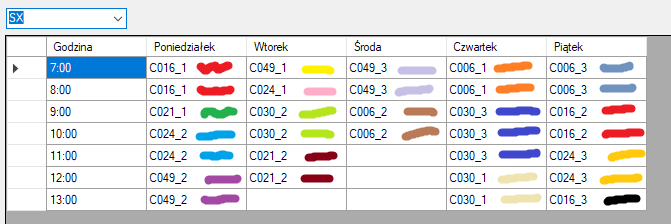
\includegraphics[width=\textwidth] {sx}
	\caption{Najlepszy otrzymany plan zajęć spośród planów dla dziesięciu klas.}
	\label{fig: sxkopia}
	\end{figure}
	
	\begin{figure}
	\centering
	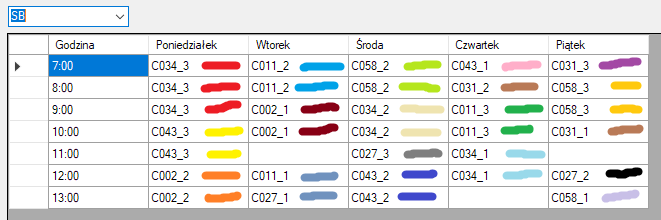
\includegraphics[width=\textwidth] {sb}
	\caption{Najgorszy otrzymany plan zajęć spośród planów dla dziesięciu klas (dwa okienka).}
	\label{fig: sbkopia}
	\end{figure}

Wykres na rysunku 7.3 przedstawia drogę algorytmu jaką musiał pokonać w czasie swojej pracy. Na osi pionowej przedstawiona jest  ocena aktualnego rozwiązania a  na osi poziomej liczba iteracji.

	\begin{figure}
	\centering
	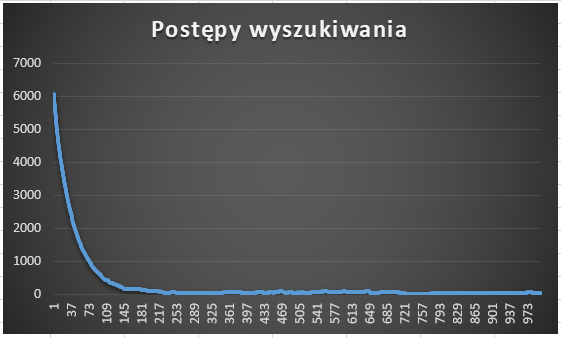
\includegraphics[width=\textwidth] {postepywyszukiwania}
	\caption{Przebieg pracy algorytmu.}
	\label{fig: postepywyszukiwania}
\end{figure}

Najlepszy wynik otrzymany został dla następujących parametrów algorytmu: liczba iteracji - 1000, czas trwania tabu - 500, rozmiar sąsiedztwa  - 300. Liczba iteracji algorytmu została ustalona, biorąc pod uwagę czas pracy programu oraz to, że liczba ta zazwyczaj wystarczała, by usunąć wszystkie konflikty z planu zajęć. 

Rozmiar sąsiedztwa również w dużej mierze wpływa na czas pracy algorytmu. Doświadczenia pokazały, że im większe sąsiedztwo tym mniej iteracji potrzebnych jest do uzyskania lepszych wyników. Rozmiar 300 to około 5\% całego sąsiedztwa możliwego do przeszukania. Przyjęcie rozmiaru sąsiedztwa na 100\%, spowodowało by wydłużenie pracy algorytmu dwudziestokrotnie. Ustalony rozmiar jest próbą pogodzenia oczekiwań, jak najkrótszego czasu pracy algorytmu i jak najlpeszych wyników.

Czas trwania tabu zmienia całkowicie sposób pracy algorytmu. Ustalenie wartości 500 wynikało z obserwacji wyników, jakie uzyskał algorytm oraz wykresów obrazujących jego pracę. Szczegółowe omówienie wpływu parametru czasu trwania tabu przedstawiono w kolejnym podrozdziale.

\section{Wpływ czasu trwania tabu na uzyskane wyniki.}

Algorytm wyszukiwania z tabu opiera się na algorytmie przeszukiwania lokalnego, w który stosuje się listę tabu. Parametr określający czas pozostawania ruchów na liście tabu ma duże znaczenie. Zmiana tego parametru powoduje zupełnie inną pracę algorytmu. Potwierdzeniem tego są wykresy przedstawione na rysunkach 7.4 - 7.8.

Na wykresach przedstawiono przebieg pracy algorytmu dla parametrów: 1000 iteracji i rozmiar sąsiedztwa równy 300. Zmieniał się tylko parametr długości tabu. Jak można zauważyć na rysunku 7.3, algorytm w początkowej fazie pracy znacznie poprawia swój wyniki (zmniejsza ocenę rozwiązania z 6000 do ok. 200). Z tego powodu na analizowanych obecnie wykresach przedstawiono tylko ostatnie 800 iteracji pracy algorytmu, by obciąć początkowy ,,skok'' i móc zaobserwować zmiany pracy algorytmu w mniejszej skali.

\begin{figure}
	\centering
	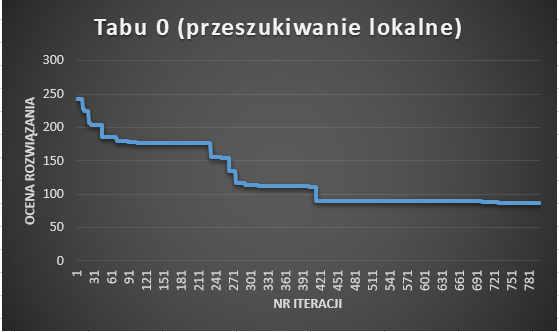
\includegraphics[width=\textwidth] {0}
	\caption{Przebieg pracy algorytmu dla czasu trwania tabu = 0.}
	\label{fig: 0}
\end{figure}

\begin{figure}
	\centering
	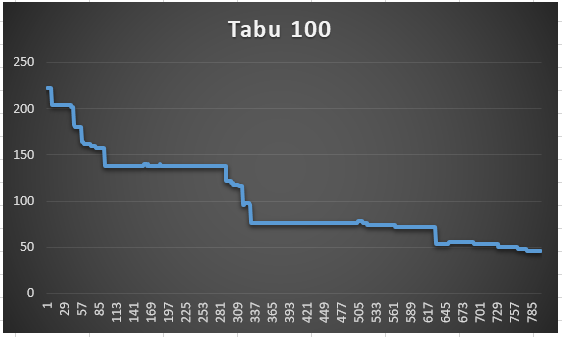
\includegraphics[width=\textwidth] {100}
	\caption{Przebieg pracy algorytmu dla czasu trwania tabu = 100.}
	\label{fig: 100}
\end{figure}

\begin{figure}
	\centering
	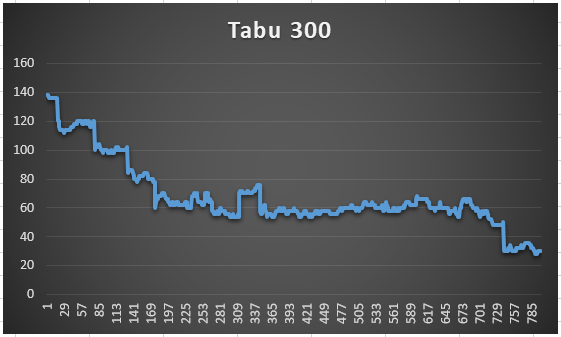
\includegraphics[width=\textwidth] {300}
	\caption{Przebieg pracy algorytmu dla czasu trwania tabu = 300.}
	\label{fig: 300}
\end{figure}

\begin{figure}
	\centering
	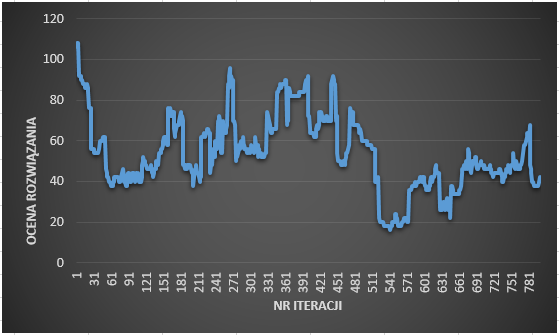
\includegraphics[width=\textwidth] {500}
	\caption{Przebieg pracy algorytmu dla czasu trwania tabu = 500.}
	\label{fig: 500}
\end{figure}

\begin{figure}
	\centering
	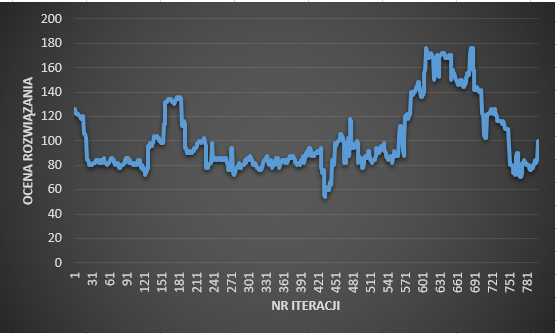
\includegraphics[width=\textwidth] {800}
	\caption{Przebieg pracy algorytmu dla czasu trwania tabu = 800.}
	\label{fig: 800}
\end{figure}

Pierwszy z wykresów (rysunek 7.4) prezentuje pracę algorytmu dla długości tabu równej 0. Oznacza to, że algorytm w ogóle nie korzysta z listy tabu. Jest to więc klasyczne przeszukiwanie lokalne. Jak widać, algorytm przeszukuje rozwiązania, które mają tą samą ocenę lub wyższą. Na wykresie nie można zauważyć skoku oceny wartości ,,w górę''. Jest to spowodowane wpadaniem algorytmu w lokalne minima, a poprawa rezultatu najczęściej jest skutkiem innego losowego wyboru sąsiadów. ocena planu jaką udało się osiągnąć to 84.

Drugi wykres (rysunek 7.5) przedstawia przebieg pracy algorytmu dla długości tabu równej 100. Otrzymany wykres jest bardzo zbliżony do poprzedniego, jednak można zaobserwować nieliczne próby pogorszenia oceny rozwiązania bierzącego w celu dotarcia do rozwiązania lepszego. Najlepszą uzyskaną oceną rozwiązania była ocena 48. Jak widać, 100 ruchów zabronionych z puli 6000 dostępnych (dla tego przypadku testowego), to zdecydowanie za mało, by efektywnie korzystać z zalet wyszukiwania z tabu.

Na trzecim wykresie (rysunek 7.6) sytuacja wygląda już zdecydowanie lepiej. Długość tabu równa 300 sprawia, że algorytm przeszukuje obszary, do których można dotrzeć tylko przez pogorszenie bieżącego wyniku. Większe skoki oceny rozwiązań to miejsca, w których udało się wyeliminować konflikt zasobów (każdy konflikt nakłada karę 20). Mniejsze zmiany obrazują próby minimalizacji okienek (każde okno czasowo powiększa ocenę rozwiązania o 2). Najlepszy uzyskany wynik to 30.

Czwarty wykres (rysunek 7.7) prezentuje sytuację, w której udało się osiągnąć najlepsze rezultaty (w tym przypadku oceną 18 - rozwiązanie optymalne to ocena 0). Najlepszy wynik udało się osiągnąć już w 740 iteracjach (540 plus 200 iteracji nie przedstawionych na wykresie). Dla długości listy tabu równej 500 przeszukiwanie odbywa się już bardzo ,,skokowo''. Algorytm nie może wykonać 500 ruchów, które w poprzednich iteracjach najbardziej poprawiły wyniki algorytmu. Musi jako bieżące rozwiązanie przyjąć rozwiązanie o gorszej ocenie. Dzięki temu jest w stanie dotrzeć do obszarów, które dla przeszukiwania lokalnego są nieosiągalne.

Ostatni wykres (rysunek. 7.8) przedstawia przebieg algorytmu dla długości tabu równej 800. Przy 1000 iteracjach tylko pierwsze 200 ruchów mogło zostać powtórzone. Niestety, tak duża liczba zabronionych ruchów spowodowała, że algorytm zdecydowanie pogorszył swoje wyniki (najlepszy rezultat to ocena 52). Choć algorytm próbował przejść w inne obszary poszukiwań, to nie otrzymano oczekiwanych rezultatów. Najprawdopodobniej, kluczowe ruchy znajdowały się na liście tabu.

\begin{figure}
	\centering
	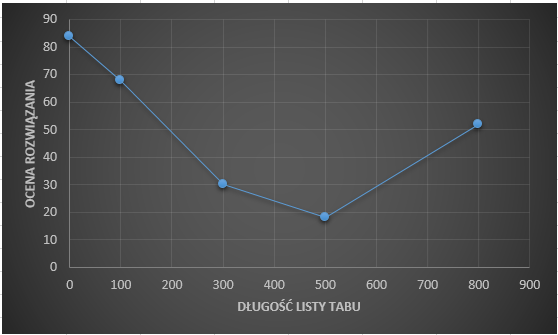
\includegraphics[width=\textwidth] {ocenadodlugosci}
	\caption{Stosunek długości listy tabu do uzyskanej oceny rozwiązania - wykres.}
	\label{fig: ocenadodlugosci}
\end{figure}

\begin{figure}
	\centering
	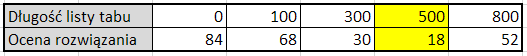
\includegraphics[width=\textwidth] {tabelaocen}
	\caption{Stosunek długości listy tabu do uzyskanej oceny rozwiązania - tabela.}
	\label{fig: tabelaocen}
\end{figure}

Rysunek 7.9 i 7.10 przedstawiają stosunek parametru długości listy tabu do otrzymanego rozwiązania. Najlepszy rezultat otrzymano dla parametru długości listy tabu równego 500. Ocena rozwiązania optymalnego, którą algorytm starał się osiągnąć jest równa 0.